\documentclass[10pt, a4paper]{article}
\usepackage{graphicx} 
\usepackage{listings}
\usepackage[table]{xcolor} 
\usepackage{amsmath}
\usepackage{amssymb}
\usepackage{wrapfig}
\usepackage{parskip}
\usepackage{float}
\usepackage[version=4]{mhchem}
\usepackage{hyperref}
\usepackage[utf8]{inputenc}
\usepackage[T1]{fontenc}
\usepackage{siunitx}
\sisetup{output-decimal-marker = {,}}
\usepackage[english]{babel}
\usepackage{array}
\usepackage{adjustbox}
\usepackage[margin=2.5 cm]{geometry}
\usepackage{appendix}
\usepackage{csquotes}
\usepackage{comment}
\usepackage{multirow}
\usepackage[
    sorting=none
]{biblatex}
\usepackage{titling}

\begin{document}

\pagenumbering{arabic}
\thispagestyle{empty}
\begin{center}
{\huge\bf Prestudy - Calibrating a Helmholtz coil and function tests of cryogenic PCB}
\end{center}
\vspace{1.0cm}
\begin{center}
Julius Berg \par
Bachelor's thesis project - \par
A cryogenic magnetic field sensor for quantum computing
\end{center}
\vspace{1.0cm}

\section{Introduction}

This prestudy presents the background theory and methodology for calibrating a constructed Helmholtz coil.
Furthermore, the coil will be used to calibrate the hall - element for later use with the entire magnetic field sensor system.

\subsection{The Helmholtz coil}
A Helmholtz coil is a pair of coils with a certaing geometry which makes it ideal for creating a homogenous magnetic field with a highly controllable magnetic flux density.
A schematic picture of the coil is shown in figure \ref{fig:helmholtz_coil}.

\begin{figure}[h]
    \centering
    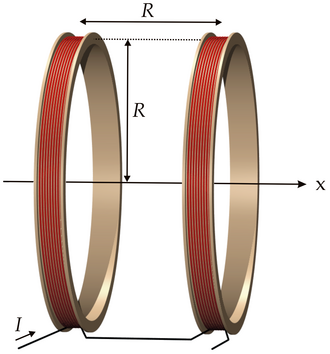
\includegraphics[width=0.3\linewidth]{Bilder/Helmholtz_coils.png}
    \caption{\textit{Schematic figure for a helmholtz coil. 
    The setup consists of two coils of equal geometry. 
    By placing the coils the same distance apart as their individual geometry,
    a homogenous magnetic field is created in the center.
    By running the same current through both coils, the magnetic flux density can be easily computed.}}
    \label{fig:helmholtz_coil}
\end{figure}

By placing the coil with a distence apart that is the same as their individual radius, the magnetic flux density in the center of the coils can be calculated as:
\begin{equation}
    B = \left(\frac{4}{5}\right)^{3/2} \frac{\mu_0 N I}{R},
    \label{eq:helmholtz_equation}
\end{equation}
with $\mu_0$ being the magnetic permeability, $N$ the number of turns per coil, $I$ the current and $R$ the radius.

The group has already counstructed a helmholtz coil. 
For this coil, the radius is $\approx$ 3 cm and each coil has aroun 100 turns (we might have lost count at some point during the winding).
The coil has been verified to conduct current and has a resistance of around 2 $\Omega$ each.
Using the geometry of our coil and expressing the magnetic flux density $B$ as a function of the current $I$,
the expression would be as follows:

\begin{equation}
    \left(\frac{4}{5}\right)^{3/2} \frac{\mu_0 N }{R} =  2.6 \cdot 10^{-3} \rightarrow B = 2.6\;I \cdot 10^{-3}
\end{equation}

We should therefore expect to see approximately $2.6 \;\si{mT/A}$ in the center of our coil.

\subsection{The Hall element}
To measure the magnetic field, a commercial Hall effect sensor is used.
The sensor is the +++ from AKM. 
It has been prepared for calibration by being mounted to a small pcb, as shown in figure

% \begin{figure}
%     \centering
%     \includegraphics[width=0.5\linewidth]{}
%     \caption{}
%     \label{fig:cryo_pcb}
% \end{figure}
By providing a current through the hall element, a measureable Hall voltage should be produced.
The formuala for the hall-voltage is given as 
\begin{equation}
    V_H = \frac{BI}{dnq}
    \label{eq:hall_voltage}
\end{equation}
with the magnetic flux denisty being $B$, the current $I$.
$d$ is the thickness of the hall element, $q$ is the charge of the charge carrier and $n$ is the charge carrier density.
Since $d$, $q$ and $n$ all are constant ($n$ changes as a function of temperature, and we can assume the temperature is constant), the hall voltage should be linearly proportional to both the magnetic flux density and the current.

Thus, by providing a steady current to our hall element we should be able to calibrate the hall voltage to the changing magnetic flux density, which we can control through our Helmholtz coil.
\section{Methodology}

\section{Expected results}
\end{document}